\documentclass[a4paper,12pt]{article}

%%% Работа с русским языком
\usepackage{cmap}					% поиск в PDF
\usepackage{mathtext} 				% русские буквы в формулах
\usepackage[T2A]{fontenc}			% кодировка
\usepackage[utf8]{inputenc}			% кодировка исходного текста
\usepackage[english,russian]{babel}	% локализация и переносы
\usepackage{xcolor}
\usepackage{hyperref}
 % Цвета для гиперссылок
\definecolor{linkcolor}{HTML}{799B03} % цвет ссылок
\definecolor{urlcolor}{HTML}{799B03} % цвет гиперссылок

\hypersetup{pdfstartview=FitH,  linkcolor=linkcolor,urlcolor=urlcolor, colorlinks=true}

%%% Дополнительная работа с математикой
\usepackage{amsfonts,amssymb,amsthm,mathtools} % AMS
\usepackage{amsmath}
\usepackage{icomma} % "Умная" запятая: $0,2$ --- число, $0, 2$ --- перечисление

%% Номера формул
%\mathtoolsset{showonlyrefs=true} % Показывать номера только у тех формул, на которые есть \eqref{} в тексте.

%% Шрифты
\usepackage{euscript}	 % Шрифт Евклид
\usepackage{mathrsfs} % Красивый матшрифт

%% Свои команды
\DeclareMathOperator{\sgn}{\mathop{sgn}}

%% Перенос знаков в формулах (по Львовскому)
\newcommand*{\hm}[1]{#1\nobreak\discretionary{}
{\hbox{$\mathsurround=0pt #1$}}{}}
% графика
\usepackage{graphicx}
\graphicspath{{pictures/}}
\DeclareGraphicsExtensions{.pdf,.png,.jpg}
\author{Бурмашев Григорий, БПМИ-208}
\title{}
\date{\today}
\begin{document}
\maketitle
\section*{Номер 10 [листок 4]}
Считаем по аналогии с семинаром:
\[
2X_1 \sim (0, 4) 
\]
\[
-3X_2 \sim (3, 9) 
\]
\[
X_3 \sim (0, 4) 
\]
\[
-X_4 \sim (-1, 4)
\]
Тогда:
\[
2X_1 - 3X_2 + X_3 - X_4 \sim (0 + 3+ 0 - 1, 4 + 9 + 4 + 4)
\]
\[
Z = 2X_1 - 3X_2 + X_3 - X_4 \sim (2, 21)
\]
Теперь:
\[
P(|Z| < 13) = P(-13 < Z < 13) = \text{Ф} \left(
\frac{13 - 2}{\sqrt{21}}
\right) - 
 \text{Ф} \left(
\frac{-13 - 2}{\sqrt{21}}
\right)  = \text{Ф} \left(
\frac{11}{\sqrt{21}}
\right) - 
 \text{Ф} \left(
\frac{-15}{\sqrt{21}}
\right)  = (\times)
\]
Посчитаем примерно:
\[
\frac{11}{\sqrt{21}} \sim  2.4 
\]
\[
\frac{-15}{\sqrt{21}} \sim -3.27
\]
\[
 \text{Ф} \left(
\frac{11}{\sqrt{21}}
\right) \sim  \text{Ф} \left(
2.4
\right) = 0.9918
\]
\[
 \text{Ф} \left(
\frac{-15}{\sqrt{21}}
\right)  =  1 - \text{Ф} \left(
\frac{15}{\sqrt{21}}
\right)  \sim 1 - \text{Ф} \left(
3.27
\right) = 1 - 0.9995 = 0.0005
\]
Тогда:
\[
(\times) \sim 0.9918 - 0.0005 = 0.9913
\]
\begin{center}
\textbf{Ответ: } 
\[
0.9913
\]
\end{center}
\clearpage
\section*{Номер 12 [листок 4]}
\begin{center}
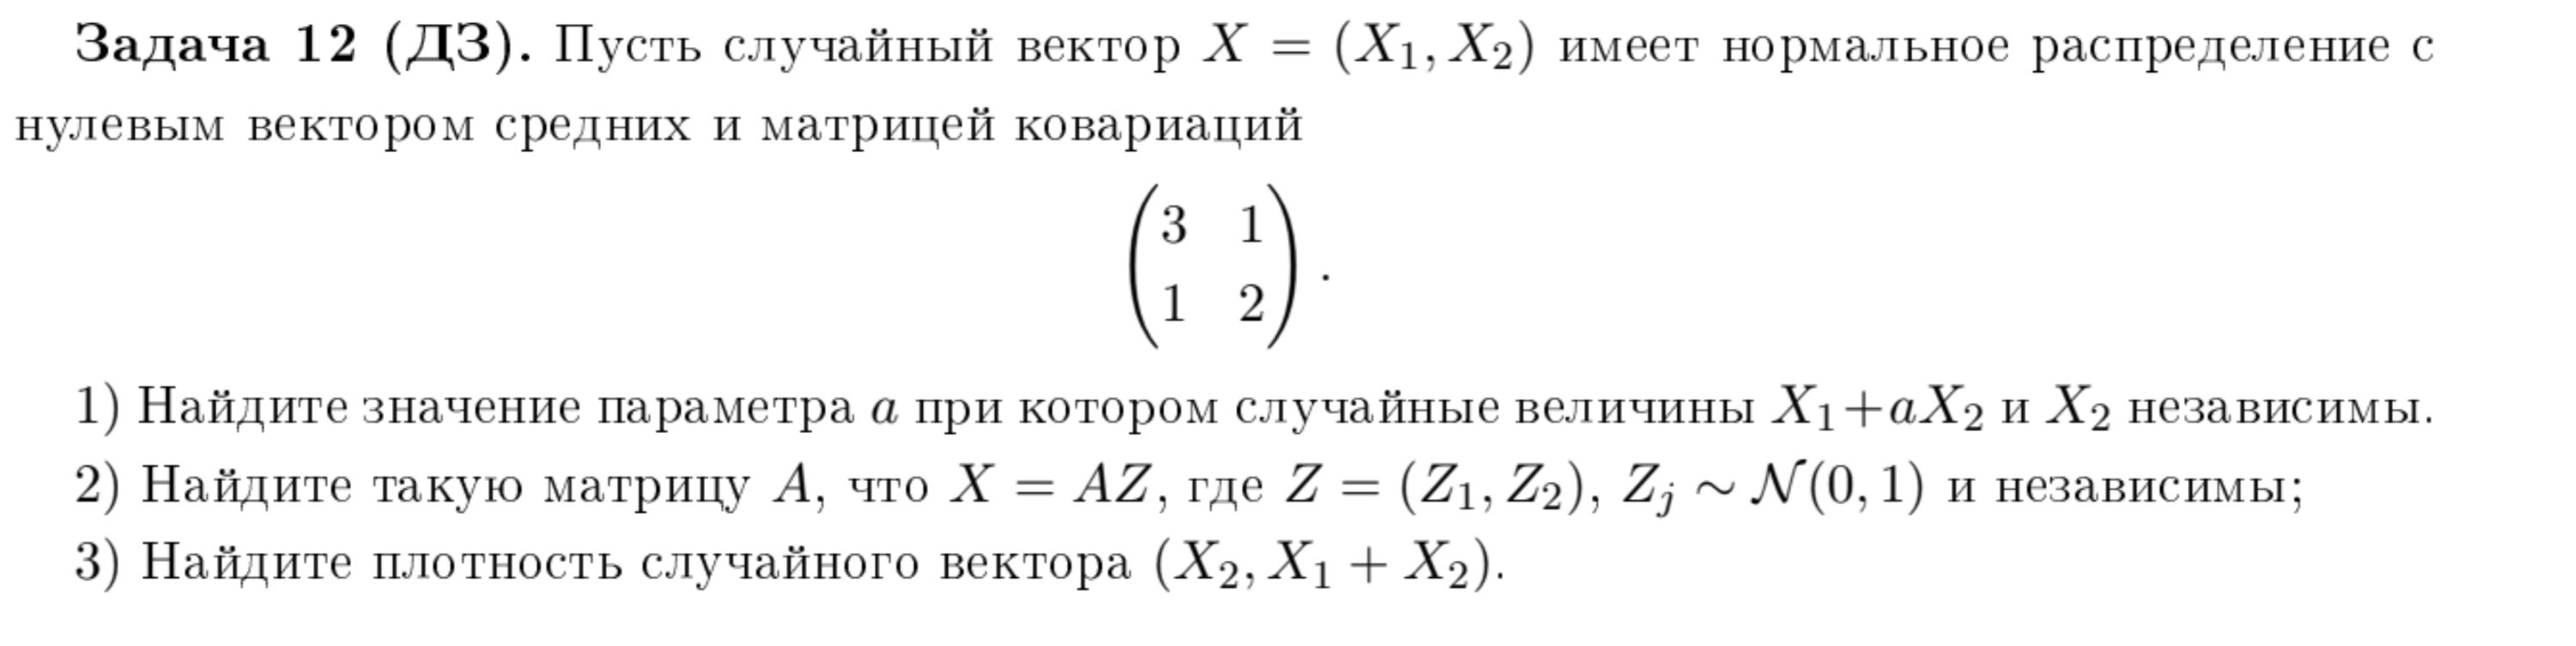
\includegraphics[scale=0.2]{1.png}
\end{center}
\subsection*{a)}
Заметим, что можем найти такую матрицу А, что вектор для наших условий будет нормальным, тобишь:
\[
Z = 
A \begin{pmatrix}
X_1 \\ X_2
\end{pmatrix}
\]
Где:
\[
A = \begin{pmatrix}
1 & a \\ 0 & 1
\end{pmatrix}
\]
Хотим (по свойствам)
\[
\text{cov} (X_1 + aX_2, X_2) = 0 
\]
Проверяем:
\[
\text{cov} (X_1 + aX_2, X_2) = \text{cov}  (X_1, X_2) + a \cdot  \text{cov }(X_2, X_2) = 1 + a \cdot 2
\]
Тогда:
\[
1 + a \cdot 2= 0
\]
\begin{center}
\textbf{Ответ: } 
\end{center}
\[
a = - \frac{1}{2}
\]
\subsection*{b)}
Аналогично семинару:
\[
Z_1 = \frac{X_1}{\sqrt{\mathbb{D}X_1}} =  \frac{X_1}{\sqrt{3}}
\]
\[
\tilde{Z_2}= X_2 - \text{cov}(X_2, Z_1) \cdot Z_1  = X_2 - \frac{1}{\sqrt{3}} \cdot 1 \cdot \frac{X_1}{\sqrt{3}} = X_2 - \frac{X_1}{3}
\]
\[
\mathbb{D} \tilde{Z_2} = \mathbb{D} \left(
X_2 - \frac{X_1}{3}
\right) = \mathbb{D}X_2 + \mathbb{D}\left(-\frac{X_1}{3}\right) + 2 \text{cov} \left(
X_2, -\frac{X_1}{3}
\right) = 2 + \frac{1}{9} \cdot 3 - 2 \cdot \frac{1}{3} \text{cov} \left(
X_1, X_2\right) = \frac{5}{3}
\]
\[
Z_2 = \frac{\tilde{Z_2}}{\sqrt{\mathbb{D}\tilde{Z_2}}} = \frac{X_2 - \frac{X_1}{3}}{\sqrt{\frac{5}{3}}} = \sqrt{\frac{3}{5}}X_2  - \sqrt{\frac{3}{5}}\frac{X_1}{3}  = - \frac{\sqrt{15}}{15}X_1 + \sqrt{\frac{3}{5}} X_2
\]
Тогда:
\[
X_1 = Z_1\sqrt{3}
\]
\[
X_2 = Z_1 \sqrt{\frac{1}{3}} + 
Z_2  \sqrt{\frac{5}{3}}
\]
А матрица:
\[
\begin{pmatrix}
X_1 \\ X_2 
\end{pmatrix} = A \begin{pmatrix}
Z_1 \\ Z_2
\end{pmatrix}  = \begin{pmatrix}
\sqrt{3} & 0 \\
\sqrt{\frac{1}{3}}& \sqrt{\frac{5}{3}}
\end{pmatrix}\begin{pmatrix}
Z_1 \\ Z_2
\end{pmatrix}  
\]
\begin{center}
\textbf{Ответ: } 
\end{center}
\[
A =  \begin{pmatrix}
\sqrt{3} & 0 \\
\sqrt{\frac{1}{3}}& \sqrt{\frac{5}{3}}
\end{pmatrix}\begin{pmatrix}
Z_1 \\ Z_2
\end{pmatrix}  
\]
\subsection*{c)}
Знаем:
\begin{center}

\includegraphics[scale=0.3]{2.png}
\end{center}
Введем:
\[
Z = \begin{pmatrix}
0 & 1 \\ 1 & 1 
\end{pmatrix} \cdot 
\begin{pmatrix}
X_1 \\ X_2
\end{pmatrix}
\]
По свойству нормального распределения ищем матрицу ковариации для Z, если у исходного X матрица была $R_1$, то для $Z$ будет:
\[
R_2 = 
AR_1A^{*} =  \begin{pmatrix}
0 & 1 \\ 1 & 1 
\end{pmatrix} \cdot \begin{pmatrix}
3  & 1\\ 1 & 2
\end{pmatrix} \cdot \begin{pmatrix}
0 & 1 \\ 1 & 1 
\end{pmatrix} = \begin{pmatrix}
2 & 3 \\ 3 & 7 
\end{pmatrix}
\]
Отсюда:
\[
\det R_2 =  14 - 9 = 5
\]
Тогда:
\[
R_2^{-1} = \left(\begin{matrix}
\frac{7}{5} & -\frac{3}{5} \\
-\frac{3}{5} & \frac{2}{5}
\end{matrix}\right)
\] 
Скалярное произведение:
\[
\begin{pmatrix}
X_1 & X_2 
\end{pmatrix}
\cdot 
\left(\begin{matrix}
\frac{7}{5} & -\frac{3}{5} \\
-\frac{3}{5} & \frac{2}{5}
\end{matrix}\right)
\cdot
\begin{pmatrix}
X_1 \\ X_2 
\end{pmatrix} = \left(
\frac{7}{5}X_1^2 - \frac{6}{5}X_1 \cdot X_2 + \frac{2}{5} X_2^2 \right)
\]
Ну и теперь тупо поставляем:
\begin{center}
\textbf{Ответ: } 
\end{center}
\[
\varrho = \frac{1}{2\pi \sqrt{5}} \cdot e^{-\frac{1}{2} \cdot \left(
\frac{7}{5}X_1^2 - \frac{6}{5}X_1 \cdot X_2 + \frac{2}{5} X_2^2 \right)}
\]
\section*{Номер 9 [листок 5]}
\begin{center}

\includegraphics[scale=0.3]{3.png}
\end{center}
\subsection*{a)}
Заметим, что $X \in (0, 1, 2)$, $Y \in (0, 1, 2, 3, 4)$, тогда в тупую заполняем табличку совместного распределения, вычисляя всевозможные исходы:
\[
P(X = 0;Y = 0) = \frac{4}{8} \cdot \frac{3}{7} \cdot \frac{2}{6}  \cdot \frac{1}{5}  = \frac{1}{70}
\]
\[
P(X = 0; Y = 1) = \frac{4}{8} \cdot \frac{3}{7} \cdot \left(
\frac{2}{6} \cdot \frac{4}{5}  +\frac{4}{6} \cdot \frac{2}{5}  
\right) = \frac{4}{35}
\]
\[
P(X = 0; Y = 2) = \frac{4}{8} \cdot \frac{3}{7} \cdot \frac{4}{6} \cdot \frac{3}{5} = \frac{3}{35}
\]
\[
P(X = 0; Y = 3) = 0
\]
\[
P(X = 0; Y = 4) = 0
\]
\[
P(X = 1; Y = 1) = \left(
 \frac{4}{8} \cdot \frac47 + \frac48 \cdot \frac47 
\right)
\cdot 
\frac36 \cdot \frac25 = \frac{4}{35}
\]
\[
P(X = 1; Y = 2) = \left(
 \frac{4}{8} \cdot \frac47 + \frac48 \cdot \frac47 
\right) \cdot \left(
\frac36 \cdot \frac35 + \frac36 \cdot \frac35 
\right) = \frac{12}{35}
\]
\[
P(X = 1; Y = 3) = \left(
 \frac{4}{8} \cdot \frac47 + \frac48 \cdot \frac47 
\right) \cdot \frac36 \cdot \frac25 = \frac{4}{35}
\]
\[
P(X = 1; Y = 4) = 0
\]
\[
P(X = 2; Y = 0) = 0
\]
\[
P(X = 2; Y = 1) = 0
\]
\[
P(X = 2; Y = 2) = \frac{4}{8} \cdot \frac{3}{7} \cdot \frac{4}{6} \cdot \frac{3}{5} = \frac{3}{35}
\]
\[
P(X = 2; Y = 3)  = \frac{4}{8} \cdot \frac{3}{7} \cdot \left(
\frac{2}{6} \cdot \frac{4}{5}  +\frac{4}{6} \cdot \frac{2}{5}  
\right) = \frac{4}{35}
\]
\[
P(X = 2; Y = 4) = 
\frac{4}{8} \cdot \frac{3}{7} \cdot \frac{2}{6}  \cdot \frac{1}{5}  = \frac{1}{70}
\]
\begin{center}
\textbf{Ответ: } 
\end{center}
\begin{center}
\renewcommand{\arraystretch}{1.5}
\renewcommand{\tabcolsep}{0.5cm}
\begin{tabular}{|c|c|c|c|}
\hline
X/Y& 0 & 1 & 2 \\
\hline
$0$ &  $\frac{1}{70}$&  $0$&$0$  \\
\hline
1 & $\frac{4}{35}$ &  $\frac{4}{35}$&  0\\
\hline
2 &$\frac{3}{35}$  &$\frac{12}{35}$  & $\frac{3}{35}$ \\
\hline
3 &  0& $\frac{4}{35}$ & $\frac{4}{35}$ \\
\hline
4 &0  & 0 & $\frac{1}{70}$ \\
\hline
\end{tabular}
\end{center}
\subsection*{b)}
Считаем по определению:
\[
\frac{P(X = 0 \cap Y = 3)}{P(Y = 3)} = 0
\]
\[
\frac{P(X = 1 \cap Y = 3)}{P(Y = 3)}  = 
\frac{\frac{4}{35}}{\frac{4}{35} +\frac{4}{35} } = \frac{1}{2}
\]
\[
\frac{P(X = 2\cap Y = 3)}{P(Y = 3)}  = 
\frac{\frac{4}{35}}{\frac{8}{35}} = \frac{1}{2}
\]
А значит:
\begin{center}
\textbf{Ответ: } 
\end{center}
\begin{center}
\renewcommand{\arraystretch}{1.5}
\renewcommand{\tabcolsep}{0.5cm}
\begin{tabular}{|c|c|c|c|}
\hline
X/Y & 0 & 1 & 2 \\
\hline
3 & 0 & $\frac12$ &$\frac12$   \\
\hline
\end{tabular}
\end{center}
\section*{c)}
\[
E(X | Y) = ?
\]
Ищем для всех $Y$ (по аналогии с семинаром):
\[
E(X | Y = 0) = \frac{1}{\frac{1}{70} + 0  + 0} \cdot \left(
\frac{1}{70} \cdot 0 + 0 \cdot 1 + 0  \cdot 2
\right) = 0
\]
\[
E(X | Y = 1) = \frac{1}{\frac{4}{35} + \frac{4}{35}} \cdot \left(
0 \cdot 0 + \frac{4}{35} \cdot 1+ 0  \cdot 2
\right) = \frac{1}{2}
\]
\[
E(X | Y = 2)  = \frac{1}{\frac{3}{35} +\frac{12}{35}  + \frac{3}{35}  } \cdot \left(
0 \cdot 0+ \frac{12}{35}  \cdot 1+ \frac{3}{35} \cdot 2
\right) = 1
\]
\[
E(X | Y = 3)  = \frac{1}{0 +\frac{4}{35}  + \frac{4}{35}  } \cdot \left(
0 \cdot 0+ \frac{4}{35}  \cdot 1+ \frac{4}{35} \cdot 2
\right) = \frac32
\]
\[
E(X | Y = 4)  = \frac{1}{0 + 0 + \frac{1}{70}} \cdot \left(
0 \cdot 0+ 0  \cdot 1+ \frac{1}{70} \cdot 2
\right)  = 2
\]
А значит:
\[
E(X | Y = y) = \frac{1}{2}\cdot y 
\]
\[
E(X | Y) = \frac{1}{2}  \cdot Y 
\]
Теперь наоборот:
\[
E(Y | X) = ?
\]
\[
E(Y | X = 0) = \frac{1}{  \frac{1}{70}+\frac{4}{35}  + \frac{3}{35}  + 0 + 0} \cdot \left(
\frac{1}{70} \cdot 0 + \frac{4}{35} \cdot 1 + \frac{3}{35} \cdot 2 + 0 \cdot 3 + 0 \cdot 4
\right) = \frac43
\]
\[
E(Y | X = 1) = \frac{1}{ 0 +  \frac{4}{35} +\frac{12}{35}  + \frac{4}{35} + 0} \cdot \left(
0 \cdot 0 + \frac{4}{35} \cdot 1 + \frac{12}{35} \cdot 2 + \frac{4}{35} \cdot 3 + 0 \cdot 4
\right) = 2
\]
\[
E(Y | X = 2) = \frac{1}{ 0  + 0 +  \frac{3}{35} +\frac{4}{35}  + \frac{1}{70} } \cdot \left(
0 \cdot 0 + 0 \cdot 1 + \frac{3}{35} \cdot 2 + \frac{4}{35} \cdot 3 + \frac{1}{70} \cdot 4
\right) = \frac83 
\]
А значит:
\[
E(Y | X = x) = \frac43 + \frac23 \cdot x
\]
\[
E(Y | X) = \frac43 + \frac23 X
\]
\begin{center}
\textbf{Ответ: } 
\[
E(X | Y) = \frac{1}{2}  \cdot Y 
\]
\[
E(Y | X) = \frac43 + \frac23 X
\]
\end{center}
\clearpage
\section*{Номер 10 [листок 5]}
\begin{center}
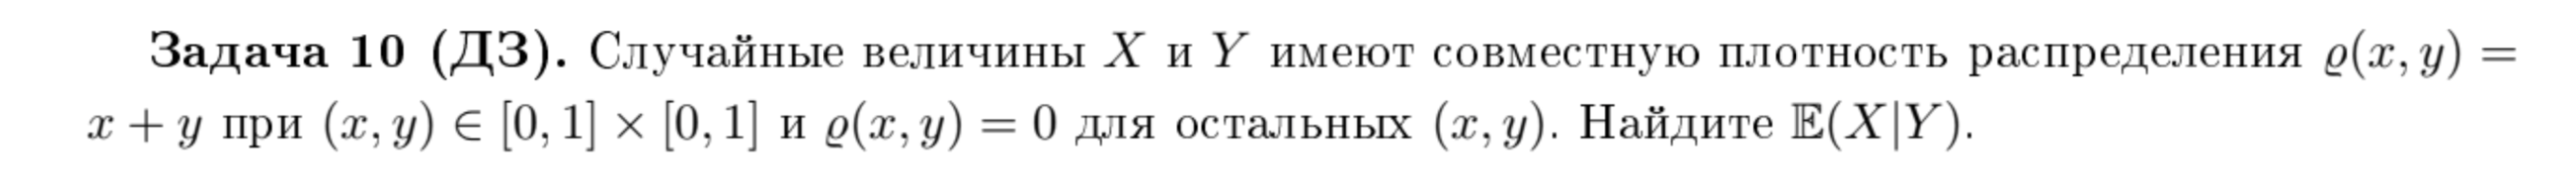
\includegraphics[scale=0.3]{4.png}
\end{center}
Знаем:
\[
E(X | Y) = \int\limits_{-\infty}^{+\infty} x \cdot \varrho_{X | Y}(x, y) dx
\]
По определению:
\[
 \varrho_{X | Y}(x, y) = \frac{ \varrho_{X,Y}(x, y)}{ \varrho_{Y}(y)}
\]
Распишем плотность из условия через индикаторы:
\[
\varrho_{X,Y}(x, y) = I_{x \in [0, 1]} \cdot I_{y \in [0, 1]} \cdot (x + y) 
\]
Еще надо найти плотность для $Y$:
\[
\varrho_{Y}(y) = \int\limits_{-\infty}^{+\infty} \varrho_{X, Y}(x, y) dx = \int\limits_{-\infty}^{+\infty}I_{x \in [0, 1]} \cdot I_{y \in [0, 1]} \cdot (x + y)  dx = 
\]
\[
= \int\limits_0^1 x \cdot I_{y \in [0, 1]} dx + \int\limits_0^1 y \cdot I_{y \in [0, 1]} dx = I_{y \in [0, 1]} \cdot \left(
\frac{1}{2}  + y 
\right) 
\]
Подставляем:
\[
 \varrho_{X | Y}(x, y)  = \frac{I_{x \in [0, 1]} \cdot I_{y \in [0, 1]} \cdot (x + y) }{I_{y \in [0, 1]} \cdot \left(
\frac{1}{2}  + y 
\right) } = \frac{I_{x \in [0, 1]} (x + y)}{\frac12 + y }
\]
Берем интеграл:
\[
E(X | Y) = \int\limits_{-\infty}^{+\infty} x \cdot \frac{I_{x \in [0, 1]} (x + y)}{\frac12 + y } dx = \frac{1}{\frac{1}{2} + y } \int\limits_{-\infty}^{+\infty} x \cdot I_{x \in [0, 1]} (x + y) dx = 
\]
\[
=
\frac{1}{\frac{1}{2} + y } \int\limits_{0}^{1} x \cdot (x + y) dx  = \frac{1}{\frac{1}{2} + y } \cdot \left(
\frac{1}{6} \cdot (3y + 2)
\right)
\]
\begin{center}
\textbf{Ответ: } 
\[
\frac{
\frac{1}{6} \cdot (3y + 2)
}{\frac{1}{2} + y } 
\]
\end{center}
\end{document}
